\section{Experimental Evaluation}

In this section, we empirically evaluate the performance of the five pricing algorithms presented 
in Section~\ref{section-approxalgo}. We evaluate the performance across two measures: $(i)$ the runtime of
the algorithm, and $(ii)$ the revenue that the algorithm can generate. 
All pricing algorithms run on hypergraph structures that are generated from a workload of
\texttt{SQL} queries executed over real-world datasets. The valuations are obtained using different
 generative models, so as to observe the algorithmic behavior under different scenarios.

%We first describe our experimental setup, followed by the various knobs that we can control to create different instances of the hypergraph instances and valuations. 

\subsection{Experimental setup}

We perform all our experiments on a $2.2$ GHz processor machine with $4$ cores and $16$ GB main memory running OS X $10.10.5$. We use \texttt{MySQL} as the underlying database for query processing and evaluation. Our implementation is written in \textsf{Python} on top of the \textsc{Qirana} query pricing system~\cite{deep2017qirana}. 
\textsc{Qirana} generates a support set $\mS$ by randomly sampling "neighboring" databases of the
underlying database $\db$, \ie databases from $\mI$ that differ from $\db$ only in a few places.
The advantage of this strategy is that it is possible to succinctly represent the support set by 
storing only the differences from $\db$, which is efficient in terms of storage.
For every query bundle $\bQ$, \textsc{Qirana} computes the conflict set $\dagr{\mS}{\bQ,\db}$, which
is the bundle (or hyperedge) that we use as input to the pricing algorithms.

Table~\ref{table:experiments} shows the design space of the experimental evaluation. 
Our experiments will be over the $\texttt{\bfseries world}$ dataset, 
and two different types of query workloads. Each query workload will generate a 
hypergraph; to assign valuations over the hyperedges, we use different generative random
models, which we describe later in detail. We evaluate our algorithms for each instance that is
generated in this fashion. 

In order to compare how well our algorithms perform in terms of revenue, we use two upper 
bounds: $(i)$ sum of valuations, and $(ii)$ an upper bound on the optimal subadditive valuation. We find an upper bound on the optimal subadditive valuations by computing a linear program whose constraints encode the arbitrage constraints. Since the number of constraints can be exponential in the number of hyperedges, we optimize by greedily adding constraints for bundles with largest valuations and finding a set of bundles that cover the hyperedge with small valuations. As we will see later, this helps us compare the performance of algorithms with respect to the subadditive bound, which can
generally be much smaller than the sum of valuations. 
In all our experiments, we report each data point as an average over $5$ runs, where we discard the first run to minimize cache latency effects on running time of the algorithms.

\begin{table*} \centering
	\def\arraystretch{1.35}%
	\begin{tabular}{c|c|c|c}
		\toprule
		\textbf{Dataset} & \textbf{Algorithms} & \textbf{Query Workload} & \textbf{Valuation Model}\\ \midrule
		$\texttt{\bfseries world}$ dataset & \ubp & uniform & sampled bundle  \\ 
		& \uip & skewed & scaled bundle  \\ 
		& \lpip &  & additive bundle  \\ 
		& \cip & &  \\
		& Layering &  &  \\
		\bottomrule
	\end{tabular}
	\caption{Experimental Design Space}
	\label{table:experiments}
\end{table*}

\subsection{Workload and Dataset Characteristics}

\begin{figure}[!h]
	\begin{minipage}[t]{0.49\linewidth} 
		\centering
		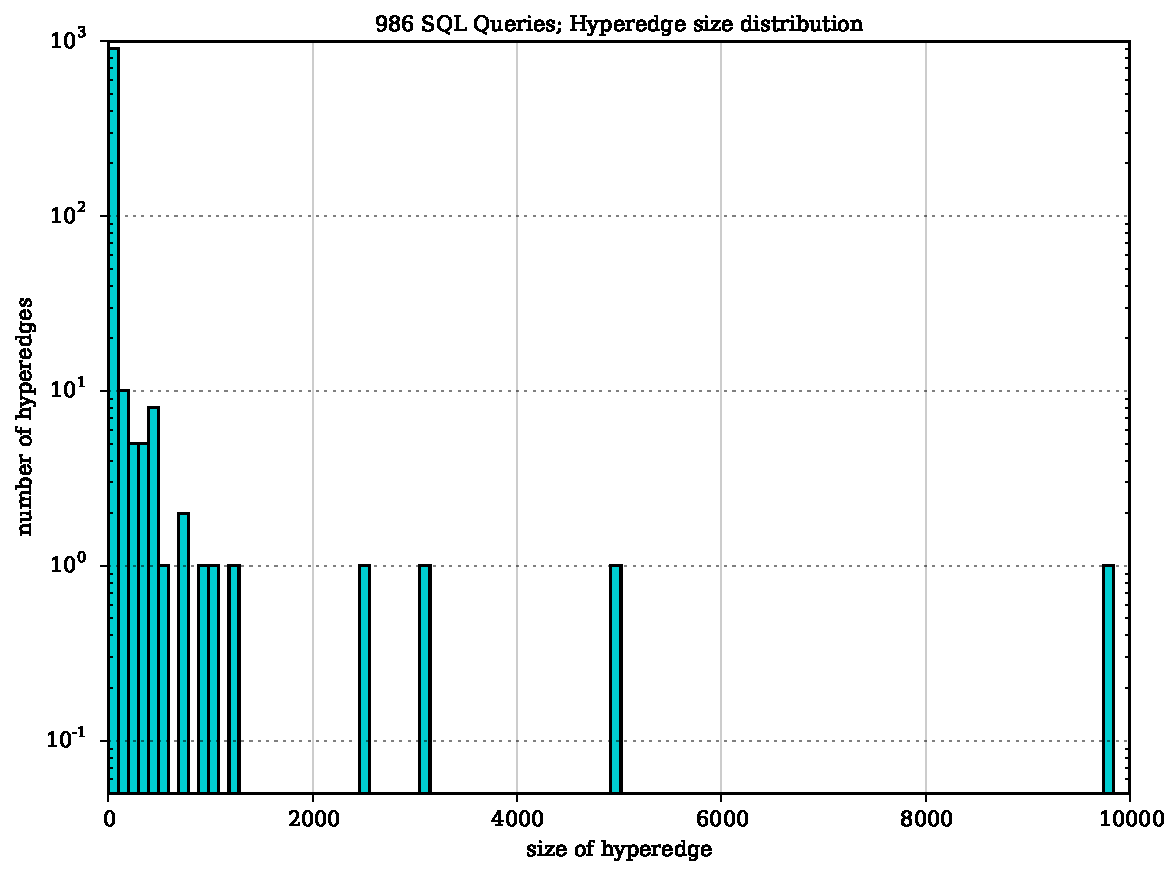
\includegraphics[scale=0.35]{histogramsqlworkload.pdf}
		\caption{Skewed query workload} \label{fig:histogramrealqueries}
	\end{minipage}       	
	%
	\begin{minipage}[t]{0.47\linewidth}
		\centering
		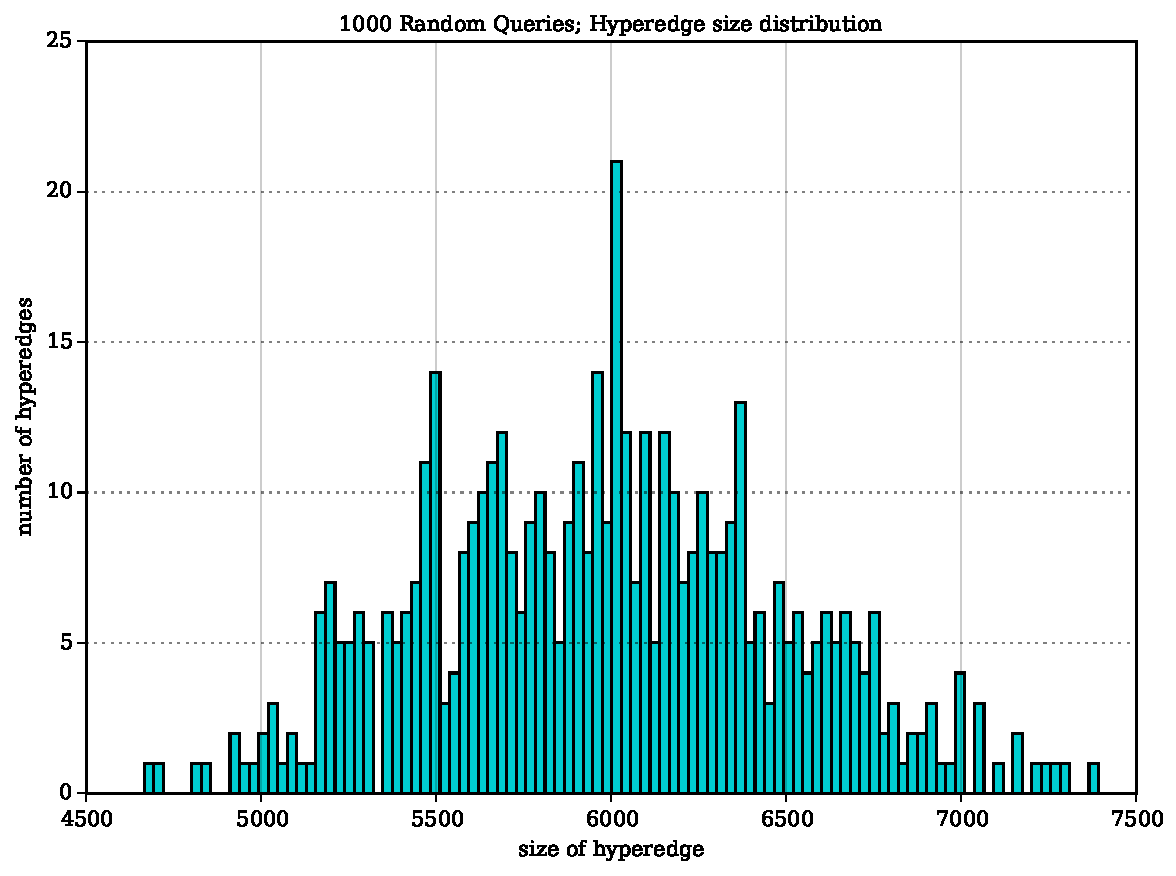
\includegraphics[scale=0.35]{histogramhyperedgesizerandomworkload.pdf}
		\caption{Uniform query workload} \label{fig:histogramrandom}
	\end{minipage} 
\end{figure}  



We now describe briefly the characteristics of the query workload and datasets. The dataset we use is the $\texttt{\bfseries world}$ dataset, a popular database provided for software developers. 
It consists of $3$ tables, which contain $5000$ tuples and $21$ attributes. We construct a support set of size $n = |\mS| = 15000$.

We consider two different query workloads, which create two different hypergraphs that fundamentally differ in structure:
%
\begin{itemize}
\item The {\em skewed} query workload consists of $m = 986$ SQL queries containing selection, projections and join queries with aggregation. The list of queries in this workload is presented in the appendix. 

%
\item The {\em uniform} query workload consists of only selection and projection SQL queries with the same selectivity (which means that the output of each query is about the same). 
%To generate a random selection query, we  sample without replacement a subset of primary keys that will included in the query. Similarly, for projection queries, we randomly choose a subset of attributes that will form the projection list of the query.
\end{itemize}



Table~\ref{table:workload:characteristics} summarizes the characteristics of the two hypergraphs
generated by each query workload. Both hypergraphs have the same number of vertices and
hyperedges. On the other hand, their structure is very different, as can be seen in 
Figures~\ref{fig:histogramrealqueries} and~\ref{fig:histogramrandom}, which depict the distribution of the hyperedge size. For the uniform query workload, the average size of each hyperedge is around 6000, and it is normally distributed around that value. This means that there is a high overlap among the vertices of the hyperedges. For the skewed query workload, most of the hyperedges contain only a very small number of vertices, while only a few hyperedges contain a large number of vertices. Observe also that the average hyperedge size is around 40, so the hypergraph is more sparse
compared to the uniform query workload.

\begin{table*}[h] \centering
	%\ra{1.3}
	\begin{small}
		\begin{tabular}{@{}lrrr@{}}\toprule
			\textbf{Query Workload} & \textbf{\# Queries ($m$)} & \textbf{Maximum item degree ($B$)} & \textbf{Average edge size} \\ \midrule
			\textbf{uniform} &  1000 & 400 & 5982.07   \\ \hdashline
			\textbf{skewed} &  986 & 22 & 41.67    \\ 
			
			\bottomrule
		\end{tabular}
	\end{small}
	\caption{Hypergraph Characteristics}
	\label{table:workload:characteristics}
\end{table*}

\subsection{Measuring the Revenue }

We first focus on the behavior of the pricing algorithms with respect to the goal of 
maximizing the revenue. We will examine separately the algorithmic behavior for
different structure of the valuations.


\subsubsection{Sampling Bundle Valuations} 
In this part of the experiment, we generate valuations for every hyperedge by sampling 
from a parametrized distribution.

First, we sample valuations from the uniform distribution $U[1,k]$ for some parameter $k$.
Figure~\ref{fig:unifzipfian} shows the performance of all five pricing algorithms. We should
remark that the revenue plotted is normalized with respect to the sum of valuations, while
the box denoted the subadditive and monotone lower bound. 
We can observe that the \lpip\ algorithm performs much better in all cases for both query
workloads. The second best algorithm is \ubp; we expect that uniform bundle pricing performs
well in this case, since the size of the bundle is not correlated with the valuation in this setup.
Finally, notice the huge gap between \uip\ and \lpip: this is an instance where both algorithms have
the same worst-case guarantees, but their revenue differs by a large margin. 

%Since the valuations for bundles are relatively close to each other, item pricing struggles to generate good prices. As we will see later, when the size of the bundle is correlated with the bundle valuation, item pricing performs much better.  

\begin{figure}[!t]
	\centering
	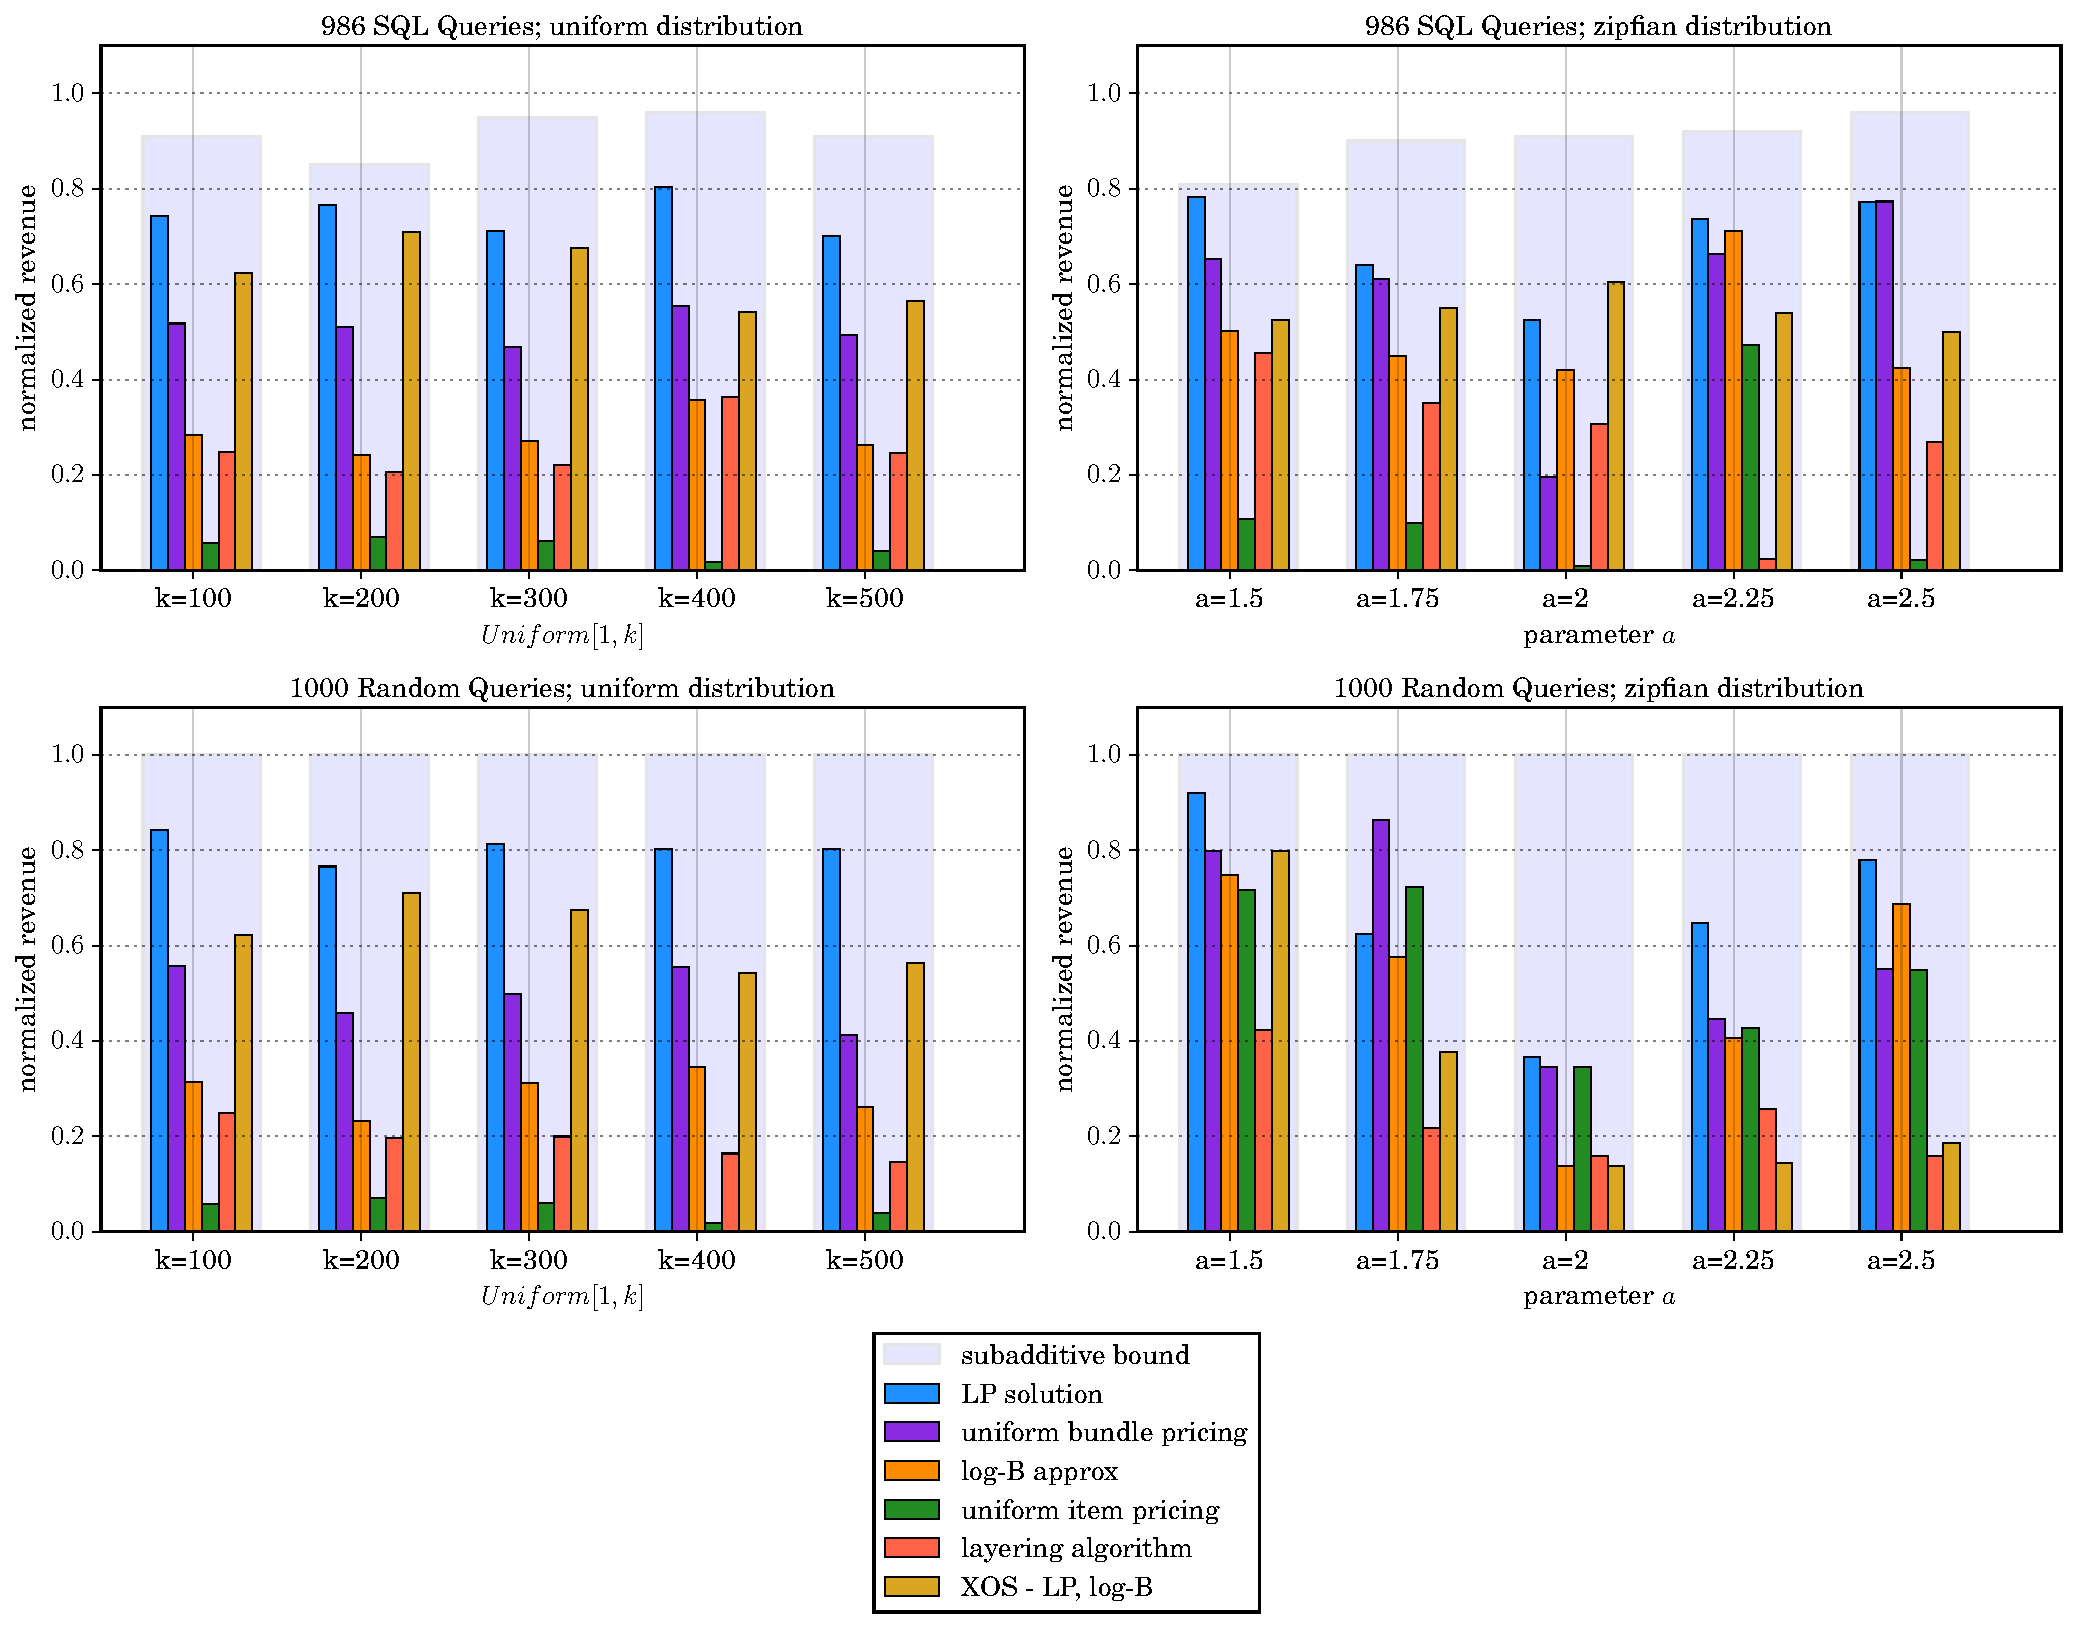
\includegraphics[scale=0.40]{uniformzipfianvaluations.pdf}
	\caption{Sampling Bundle Valuations: uniform and skewed workload} \label{fig:unifzipfian}
\end{figure}  

Second, we sample valuations from the zipfian distribution parametrized by $a$.
\lpip\ again performs better than the other pricing algorithms, but now \ubp\ comes a close second
(and in one case performs better than \lpip).  

The layering algorithm does not perform well except in the case of zipfian distribution with exponent smaller than $2$. Indeed, for $a < 2$, zipfian distribution assigns a large valuation to some hyperedge that contributes significantly to the total revenue. In such cases, the layering algorithm can always extract full revenue from the layer containing high valuation edges and perform well in practice. As the zipfian exponent becomes greater than two, the spread of valuations becomes smaller and the layering algorithm performs worse. 

Finally, the \cip\ algorithm does not perform that well, even though it is theoretically optimal. This is because going over all capacity vectors with limited supply is extremely expensive. In our implementation, running the linear program for a large number of capacity vectors for the uniform workload takes close to $2$ hours in total (we discuss reasons for this in the next section). Thus, we reduce the number of capacity vectors that we try by increasing the $(1+\epsilon)$ parameter. This introduces a factor of $(1+\epsilon)$ in the approximation ratio but allows for the running time to be smaller. For the purpose of experiments, we set $(1+\epsilon)$ such that the running time is $\sim 30$ minutes. Performing this optimization allows us to complete the algorithm rather than truncating the experiment prematurely and returning the best result obtained so far.  The approximation factor of \cip\ remains marginally inferior to \lpip (although in some cases, it outperforms \lpip). 


\begin{figure}[!t]
	\centering
	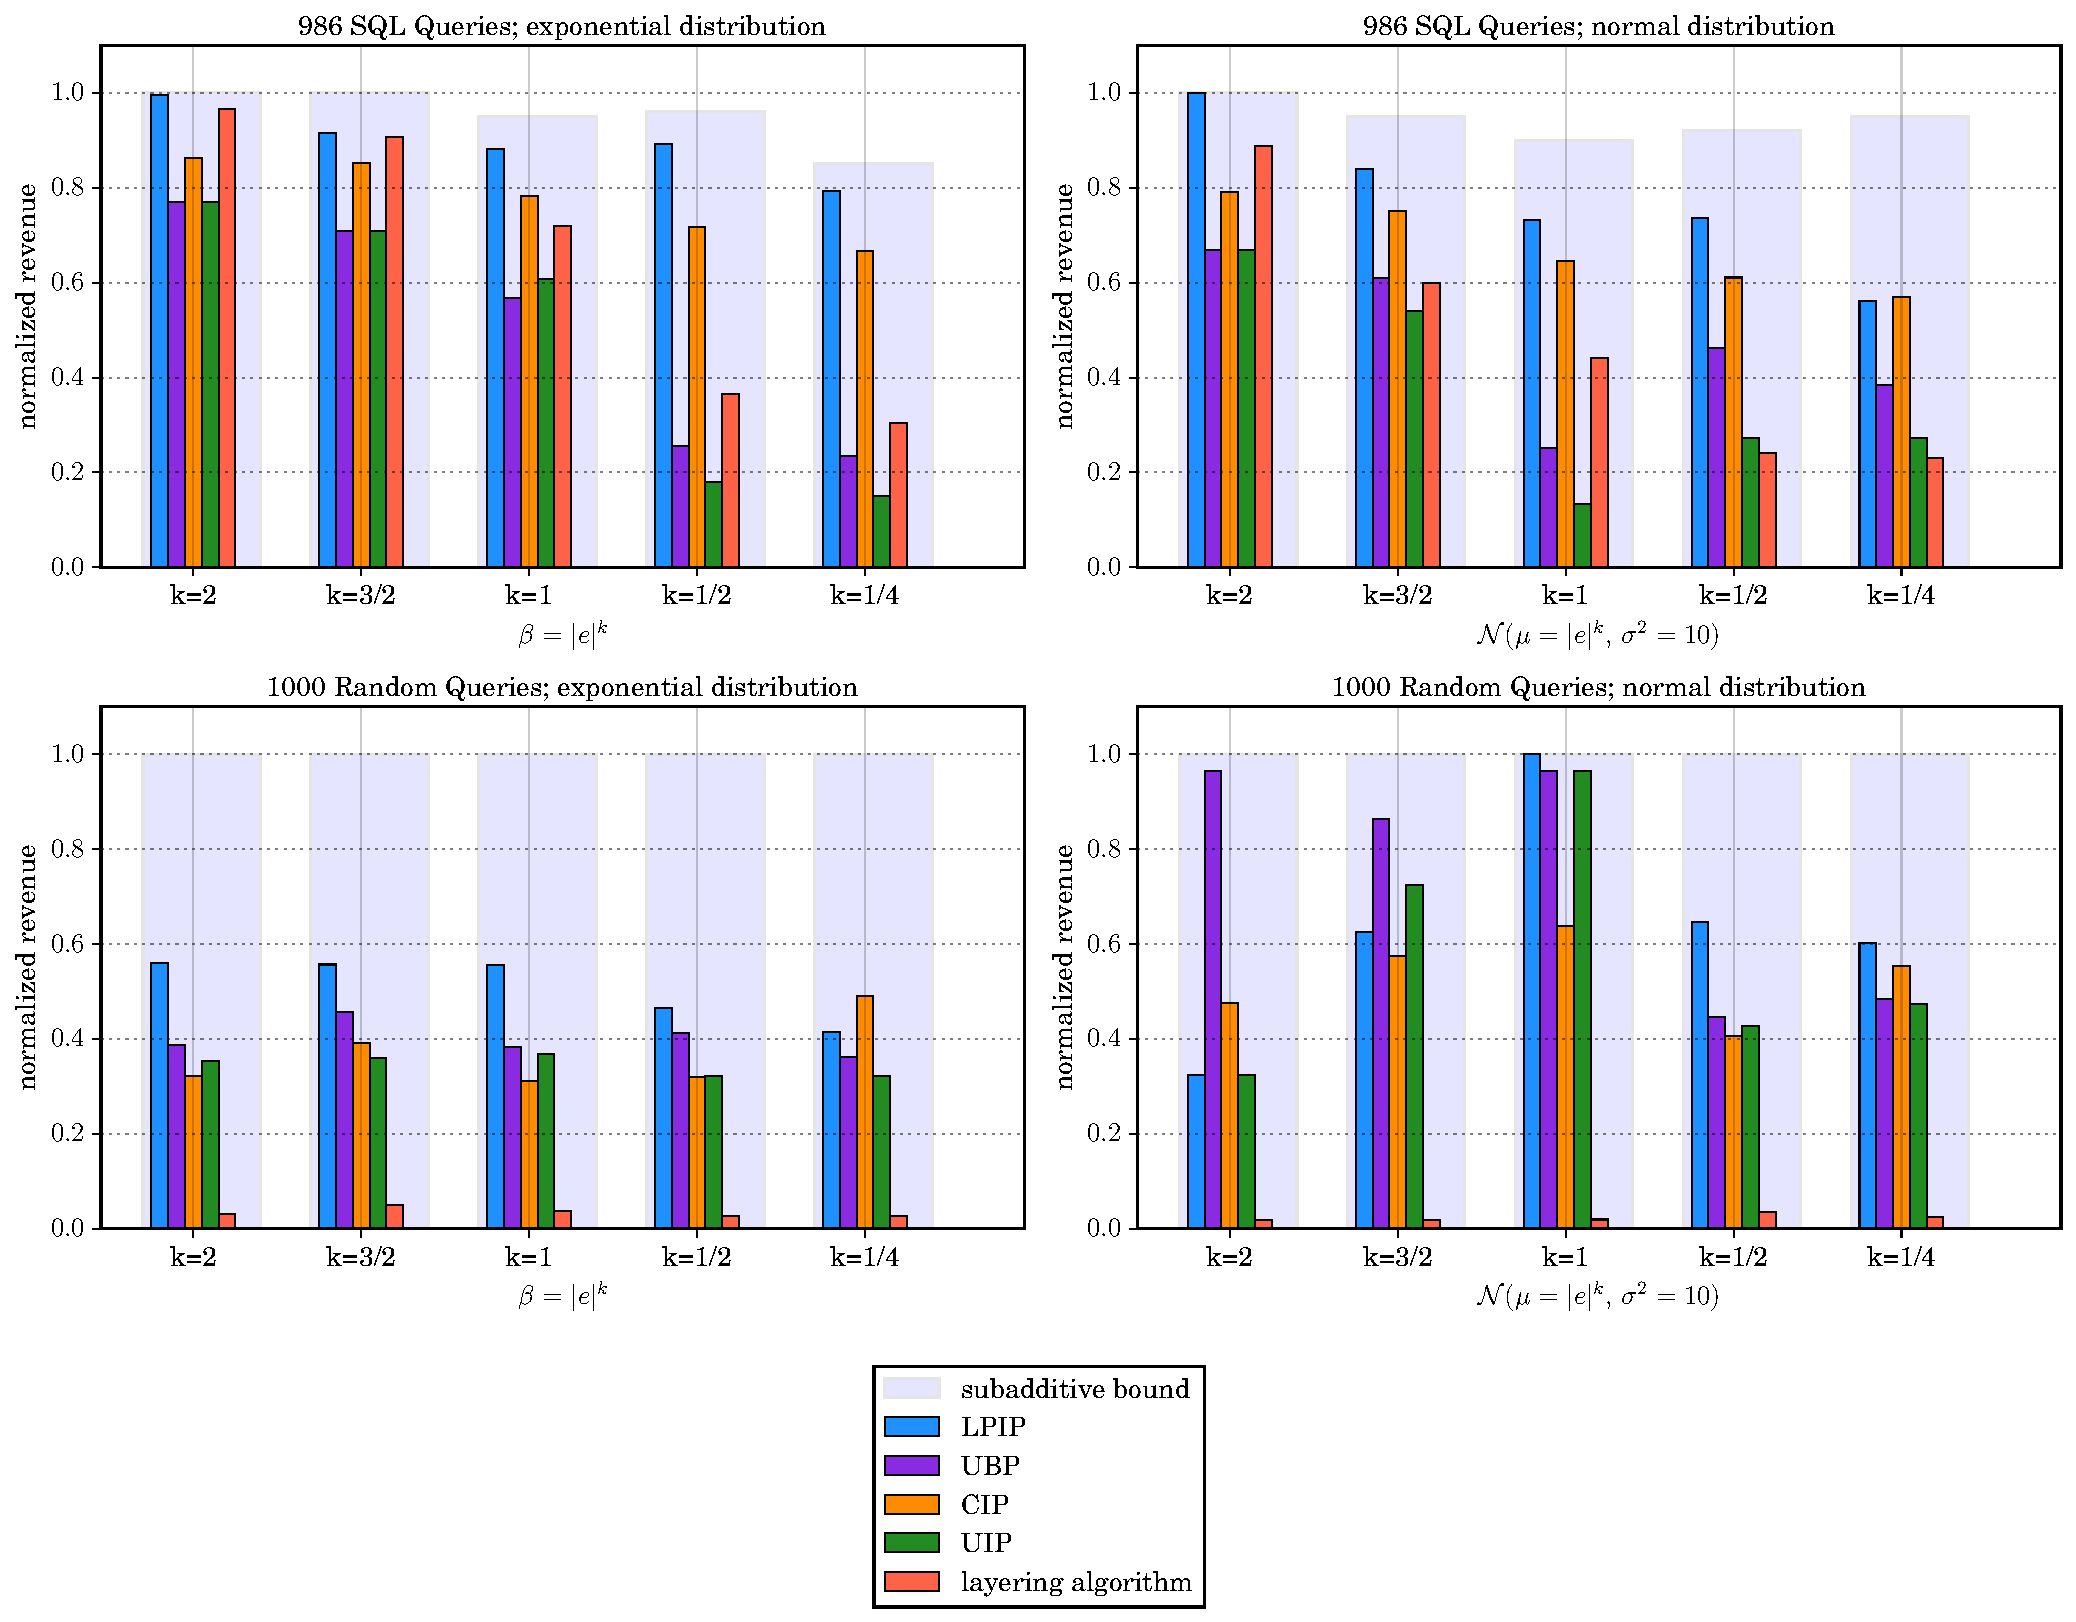
\includegraphics[scale=0.40]{queriesscalingedgesize.pdf}
	\caption{Scaling Bundle Valuations: uniform and skewed workload} \label{fig:scalingedge}
\end{figure}  

\subsubsection{Scaling Bundle Valuations} In the previous, the valuations are sampled independently of the edge size. Our next experiment correlates the size of each hyperedge with the valuation that is assigned to it. 
To achieve this, we sample each valuation from the parameterized exponential and normal distribution as follows: we assign $v_e \sim {\rm exponential} (\beta = m^k)$ where $\beta$ is the mean of the distribution. Similarly, for normal distribution, we assign $v_e \sim \mathcal{N}(\mu = m^k,\, \sigma^2 = 10)$. Here $k$ is the parameter that we will vary. Figure~\ref{fig:scalingedge} shows the revenue
generated for the two query workloads and two families of distributions for 
different values of the parameter $k$. 

For the skewed query workload, when $k \geq 1$, most of the revenue is concentrated in a few edges that have extremely large valuations (because there are few edges of large size). In this case, all
algorithms perform very well and extract almost all of the revenue. For smaller values of $k$, the algorithms can extract smaller revenue, and \lpip\ and \cip\ perform best. Notice again the large revenue gap between \lpip\ and \uip\ for such values (as much as 5x).

The landscape changes for the uniform query workload. The main observation is that the layering
algorithm performs extremely poorly. The revenue generated by the other four algorithms is very
close, with \lpip\ and \ubp\ performing the best.  
For the exponential distribution, all algorithms are very far from optimal. However, we believe this is not an anomaly but rather the subadditive bound not being as good as it should be.


\begin{figure}[!t]
	\centering
	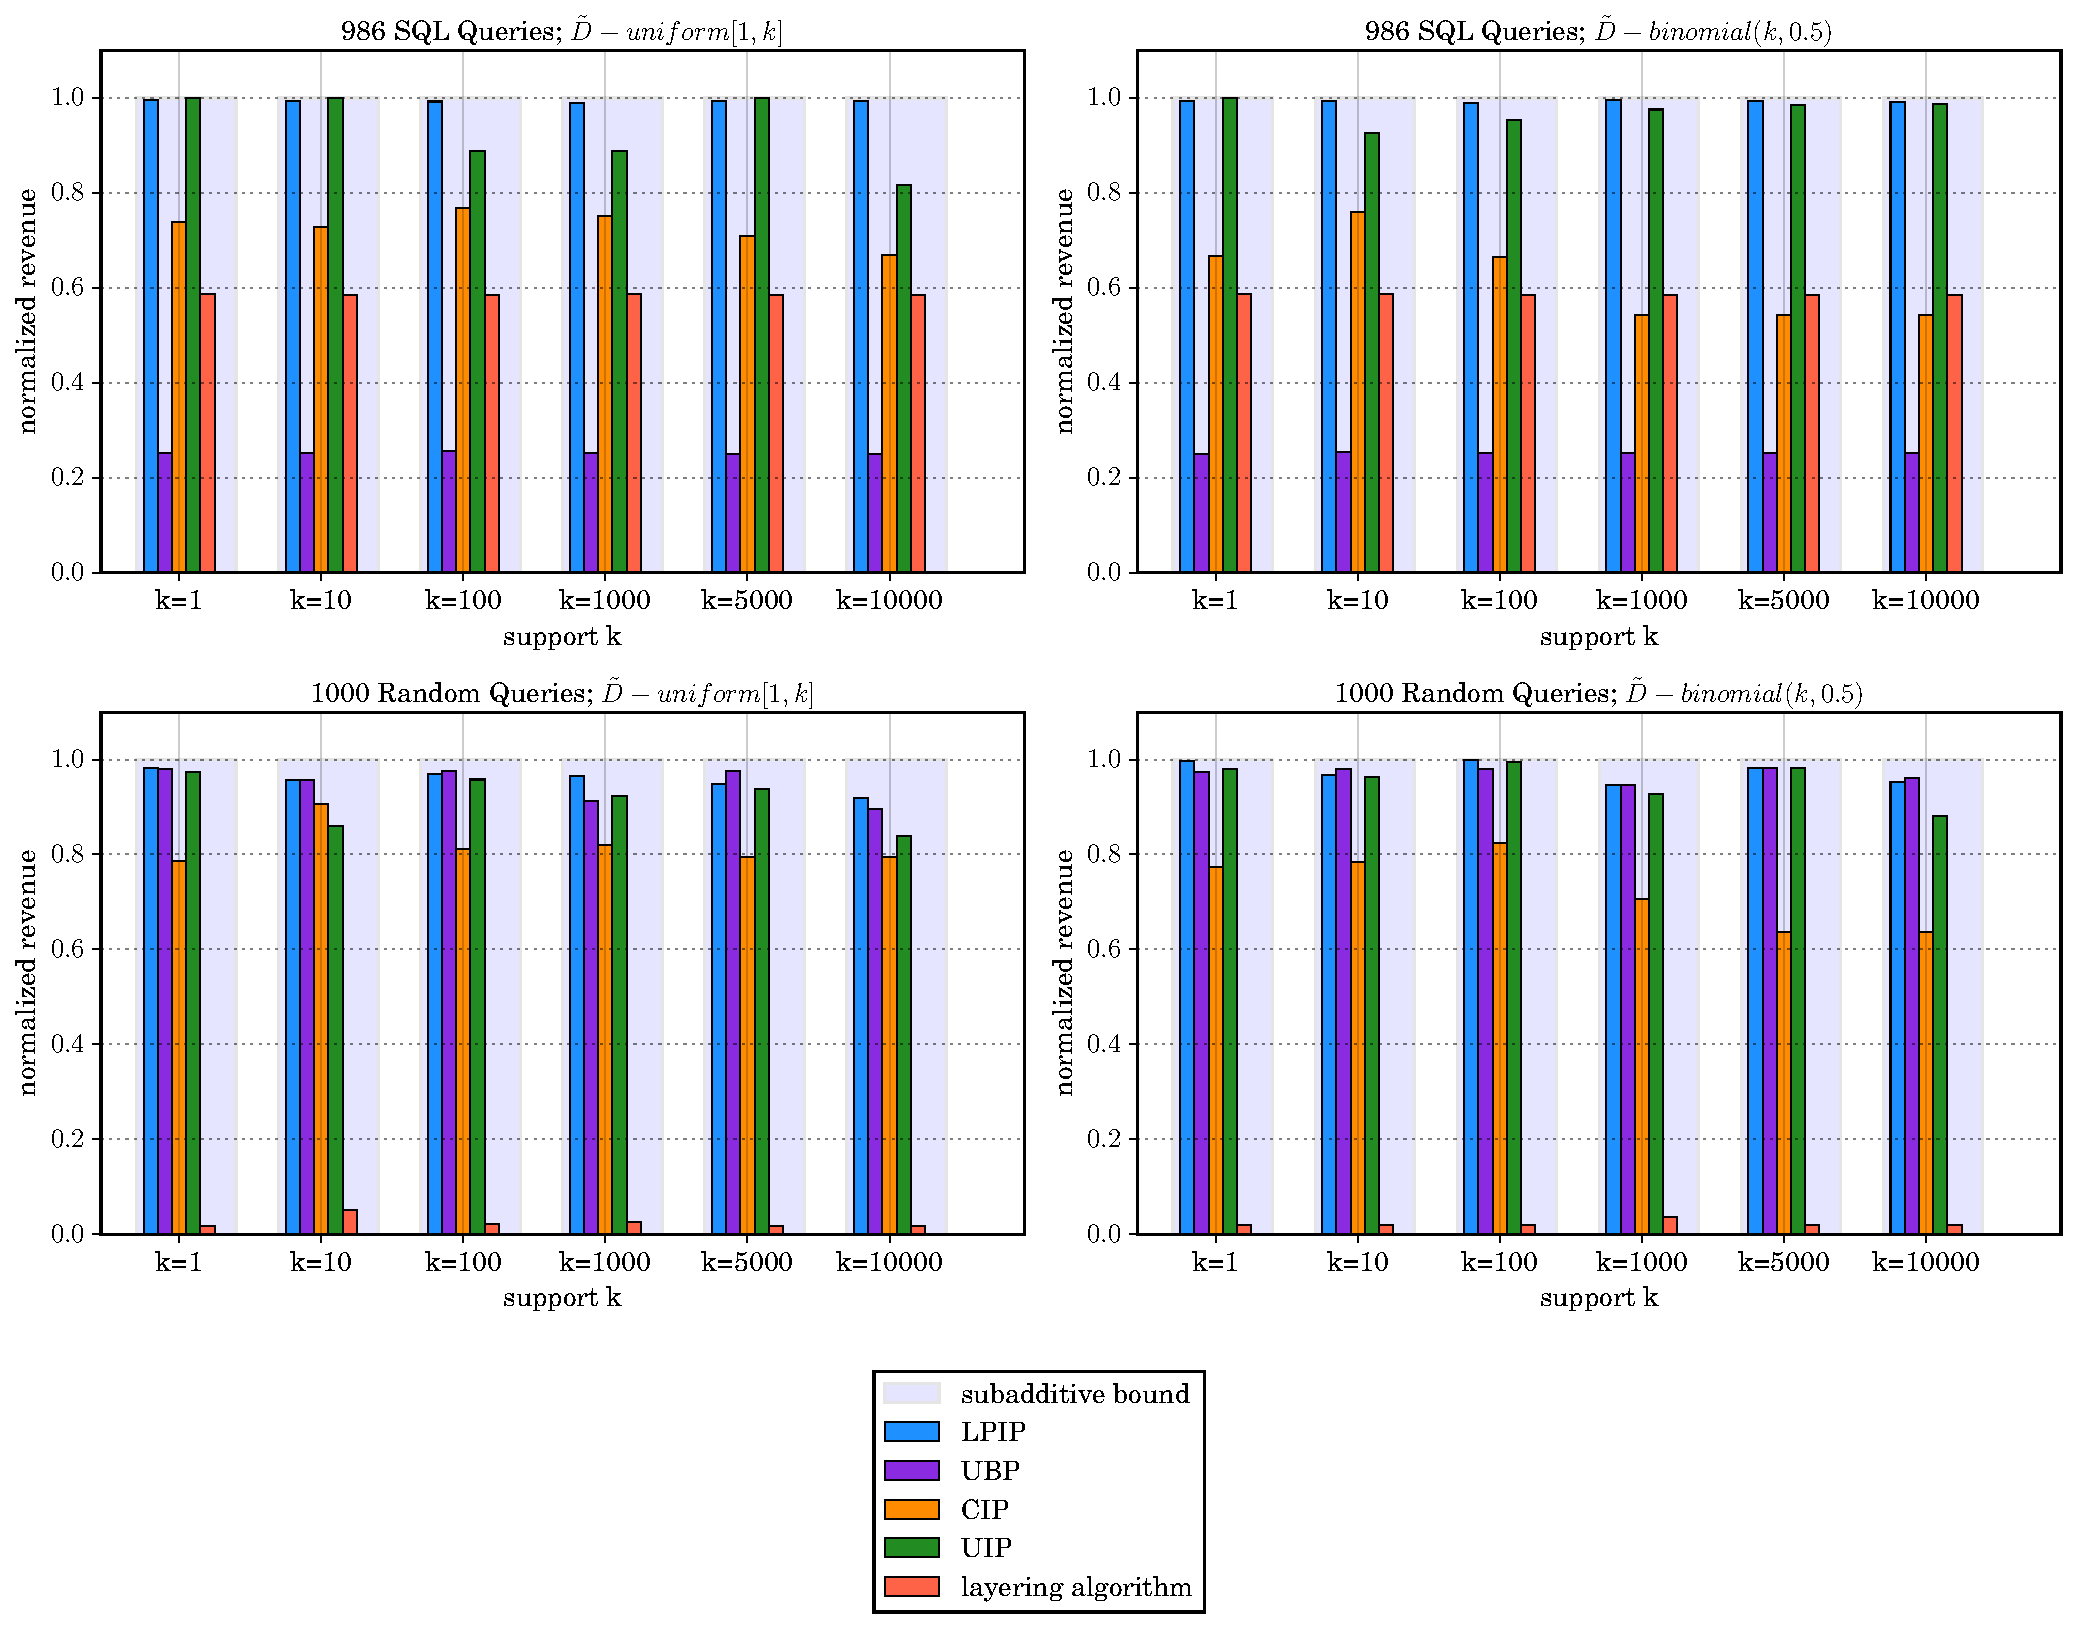
\includegraphics[scale=0.40]{queriesmixing.pdf}
	\caption{Sampling Item Prices: uniform and skewed workload} \label{fig:mixing}
\end{figure}  

\subsubsection{Sampling Item Prices} The last of set of experiments is to understand the behavior of the pricing algorithms when the valuation of each hyperedge is defined by an \emph{additive generative model}. More specifically, we define $k$ different distributions $\{D_i\}_{i=1}^{k}$ from which items will draw their prices and a special distribution $\tilde{D}$ which will assign each item which distribution it will sample from. The valuation of an edge is the defined as $v_e = \sum_{j \in e} x_j \sim D_{\ell_j}$ where $\ell_j \sim \tilde{D}$. Intuitively, this model will capture the scenario where parts of the database have non-uniform value and some parts are much more valuable than others. To see why this setting can be practical interest, consider a research analyst in banking who gives stock recommendations. While public information about companies and stocks may be cheap, the research analysts buy and sell recommendations will be of much higher value. For the purpose of experiments, we fix $D_i$ to $\textsf{Uniform}[i, i+1]$ and set $\tilde{D}$ to $\textsf{Uniform}[1, k]$ or $\textsf{Binomial}(k, 1/2)$ while varying $k$. Figure~\ref{fig:mixing} shows the results of this experiment. 

Here, \lpip\ outperforms all other algorithms. For small values of $k$, the valuation of each hyperedge is closer to $|e|$. In this case, there is no gap between \uip\ and its \lpip. As the value of $k$ increases, the gap between the two algorithms increases, since the weights of each item become less uniform.
 
We should remark two things that are distinct for each query workload. For the skewed query workload, \ubp\ performs poorly, since now the valuation of each hyperedge is correlated (in an additive fashion) with the bundle structure. For the uniform query workload on the other hand, \ubp\ does well, since   
the size of the edges is relatively concentrated. Finally, the layering algorithm is the worst performing out of all in the case of the uniform query workload.

\subsection{Measuring the Runtime}

\begin{table*}[] \centering
	%\ra{1.3}
	\begin{small}
		\begin{tabular}{@{}lrrrrr@{}}\toprule
			\textbf{Query Workload} & \textbf{\lpip} & \textbf{\ubp} & \textbf{\uip} & \textbf{\cip} & \textbf{Layering}  \\ \midrule
			
			\textbf{skewed} &  60.62 & 15.50 & 25.45 & 812.67 & 15.67 \\ \hdashline
			\textbf{uniform} &  95.81 & 18.68 &  29.82 &1800 & 50.19 \\
			\bottomrule
		\end{tabular}
	\end{small}
	\caption{Algorithm running times (in seconds) for different workloads.}
	\label{table:runtime}
\end{table*}

In this section we discuss the running time of the algorithms. Table~\ref{table:runtime} shows the runtime of all algorithms for both query workloads. The most time efficient algorithms are uniform bundle pricing, uniform item pricing and the layering algorithm. Uniform bundle pricing and uniform item pricing depend only on number of hyperedges and the number of items in the hypergraph. Thus, they are very fast to run in practice. The layering algorithm is slightly slower but comparable in performance. Note that the layering is faster on the skewed query workload as compared to the uniform query workload, since the maximum degree $B$ is much smaller. 

The two slowest running algorithms are \lpip\ and \cip\ as they require running multiple linear programs. In practice, \lpip\ is faster than \cip. This is because the size of the linear program is very different. In our setting, the number of edges $m \sim 1000$ is much smaller than the number of items $n = 15000$. \lpip\  has at most one constraint per bundle (thus, at most $m$ constraints) but \cip\ has one constraint per item ($n$ constraints in total). This dramatically influences the running time of the two algorithms. \cip\ uses $(1+\epsilon)$ as a parameter, where $\epsilon$ controls the limited supply available for each item. We adjust the value of $\epsilon$ for both workloads to ensure that the running time is at most $30$ minutes. We fix $\epsilon = 0.2$ for the skewed workload and $\epsilon = 4$ for the uniform workload based on our empirical observations.


\subsection{Impact of Support Set Size}


\begin{figure}[!t]
	\centering
	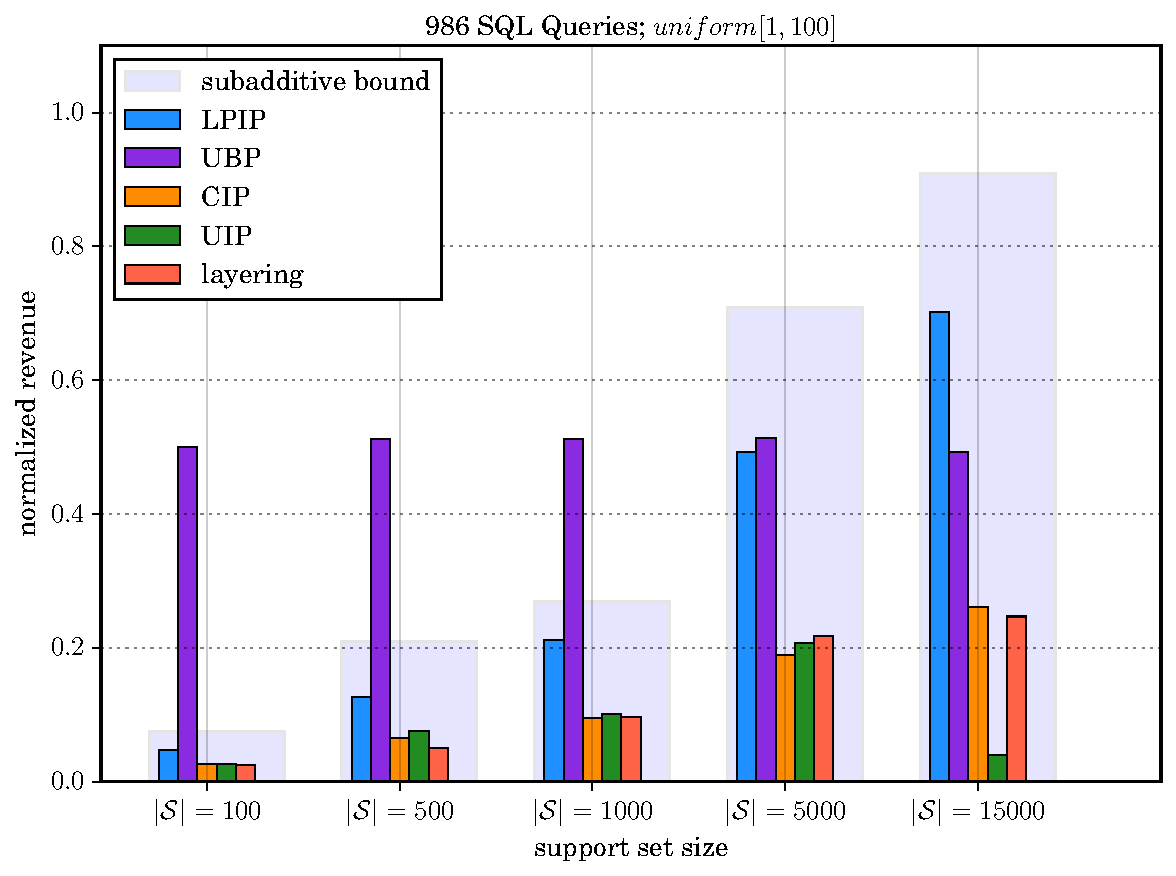
\includegraphics[scale=0.40]{varyingsupportset.pdf}
	\caption{Revenue generated with changing item set} \label{fig:supportsetsize}
\end{figure}  

\begin{table*}
	\begin{small}
		\begin{tabular}{@{}lrrrrr@{}}\toprule
			\textbf{Support Set Size} & \textbf{\lpip} & \textbf{\ubp} & \textbf{\uip} & \textbf{\cip} & \textbf{Layering}  \\ \midrule
			
			$|\mS| = 100$ &  $<1$ & $<1$ & $<1$ & $<1$ & $<1$ \\ \hdashline
			$|\mS| = 500$ &  6.16 & 4.32 &  5.25 & 6.87 & $<1$ \\ \hdashline
			$|\mS| = 1000$ &  15.10 & 8.71 &  17.43 & 29.82 & $<1$ \\ \hdashline
			$|\mS| = 5000$ &  30.12 & 18.68 &  29.82 & 189.97 & 3.65 \\ \hdashline
			$|\mS| = 15000$ &  70.42 & 25.19 &  35.21 & 676.23 & 12.34 \\
			\bottomrule
		\end{tabular}
	\end{small}
	\caption{Algorithm running times (in seconds) for skewed workload}
	\label{table:runtime:supportsetsize}
\end{table*}

Our final set of experiments is to understand the impact of support set size, i.e, the number of items $n$. Given a hypergraph instance, adding more items to the hypergraph is an interesting propositions since it can only increase the revenue. However, this also comes at a higher cost of algorithm running time. On the other hand, too few items in the hypergraph can lead to bad revenue generation for most algorithms (except uniform bundle pricing since it is independent of the items). Figure~\ref{fig:supportsetsize} demonstrates the impact of changing support set size on the revenue extracted. Unsurprisingly, uniform bundle pricing is not impacted by the support set size. As the support set size decreases for $15000$ to $100$, the subadditive bound also decreases which caps the performance of all item pricing algorithm. Table~\ref{table:runtime:supportsetsize} depicts running time of all algorithms as a function of support size. The key takeaway is that running time is dependent on the support set size. Thus, the right tradeoff depends on the data seller requirements. It remains an interesting open problem to design algorithms for choosing the items in a smarter way. This will ensure that we can get good revenue guarantees without sacrificing running time too much.

